\apendice{Documentación de usuario}

\section{Introducción}
En este apartado se explica la información que puede resultar de interés al usuario. Este apartado está escrito para entender lo que ofrece eLearningQA y como se usa.
\section{Requisitos de usuarios}
Para poder utilizar la aplicación es necesario disponer de una cuenta de Moodle con permisos de profesor y profesor sin permisos de edición o superior.

Además, es necesario de disponer de conexión a internet para acceder a la página web en la que está la aplicación
\section{Instalación}
eLearningQA no requiere de instalación, ya que es una aplicación web.
\section{Manual del usuario}
\subsection{Pantallas}
    \begin{itemize}
        \item \textbf{Inicio de sesión:} La primera pantalla que el usuario puede ver es la de inicio de sesión \ref{fig:pantalla-inicio}. En esta encontramos un formulario para introducir las credenciales, la url de la página de Moodle, y el fichero de configuración.
        Además, se puede ver un footer que muestra los botones para acceder al manual de usuario, a la información de la aplicación y para el contacto con el responsable de la web.
        \begin{figure}[H]
            \centering
            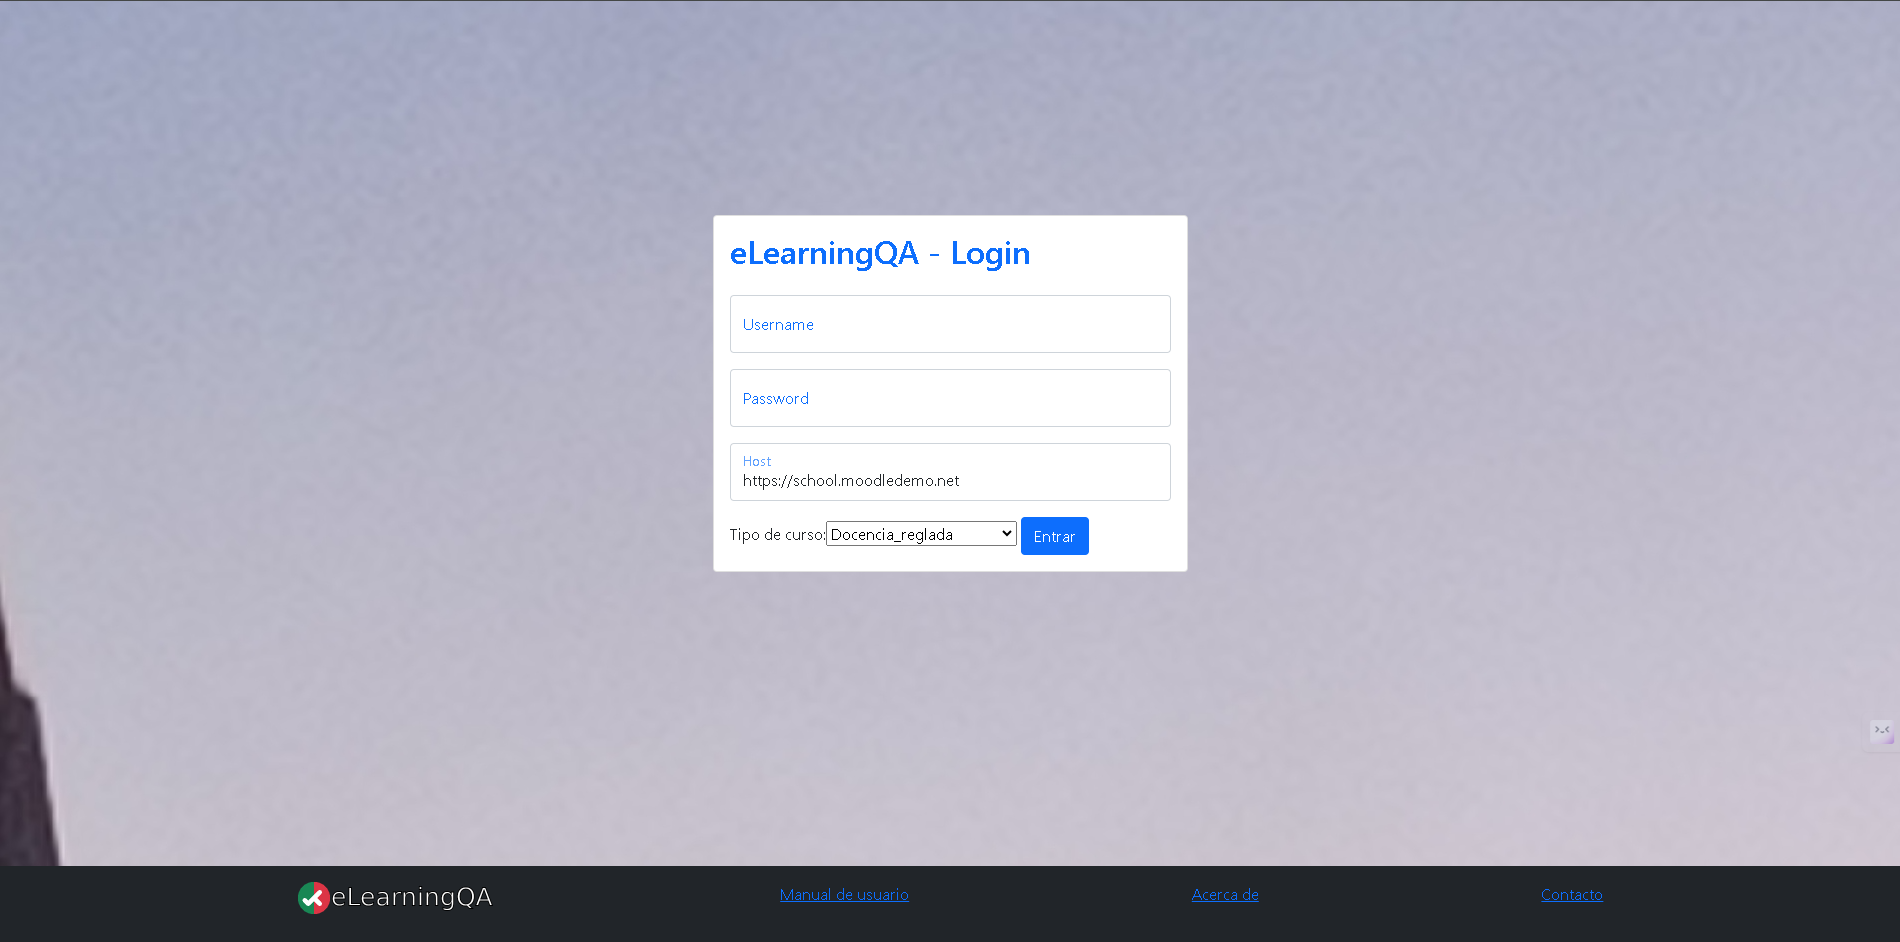
\includegraphics[width=1\linewidth]{img/incio-sesion.png}
            \caption{Pantalla de inicio de sesión}
            \label{fig:pantalla-inicio}
        \end{figure}
        \item \textbf{Lista de cursos:} Una vez iniciada la sesión se podrá visualizar una lista de cursos \ref{fig:lista-cursos} de los que se puede obtener un informe de calidad. Además, se puede ver un botón de desconexión para salir de la aplicación.
        \begin{figure}[H]
            \centering
            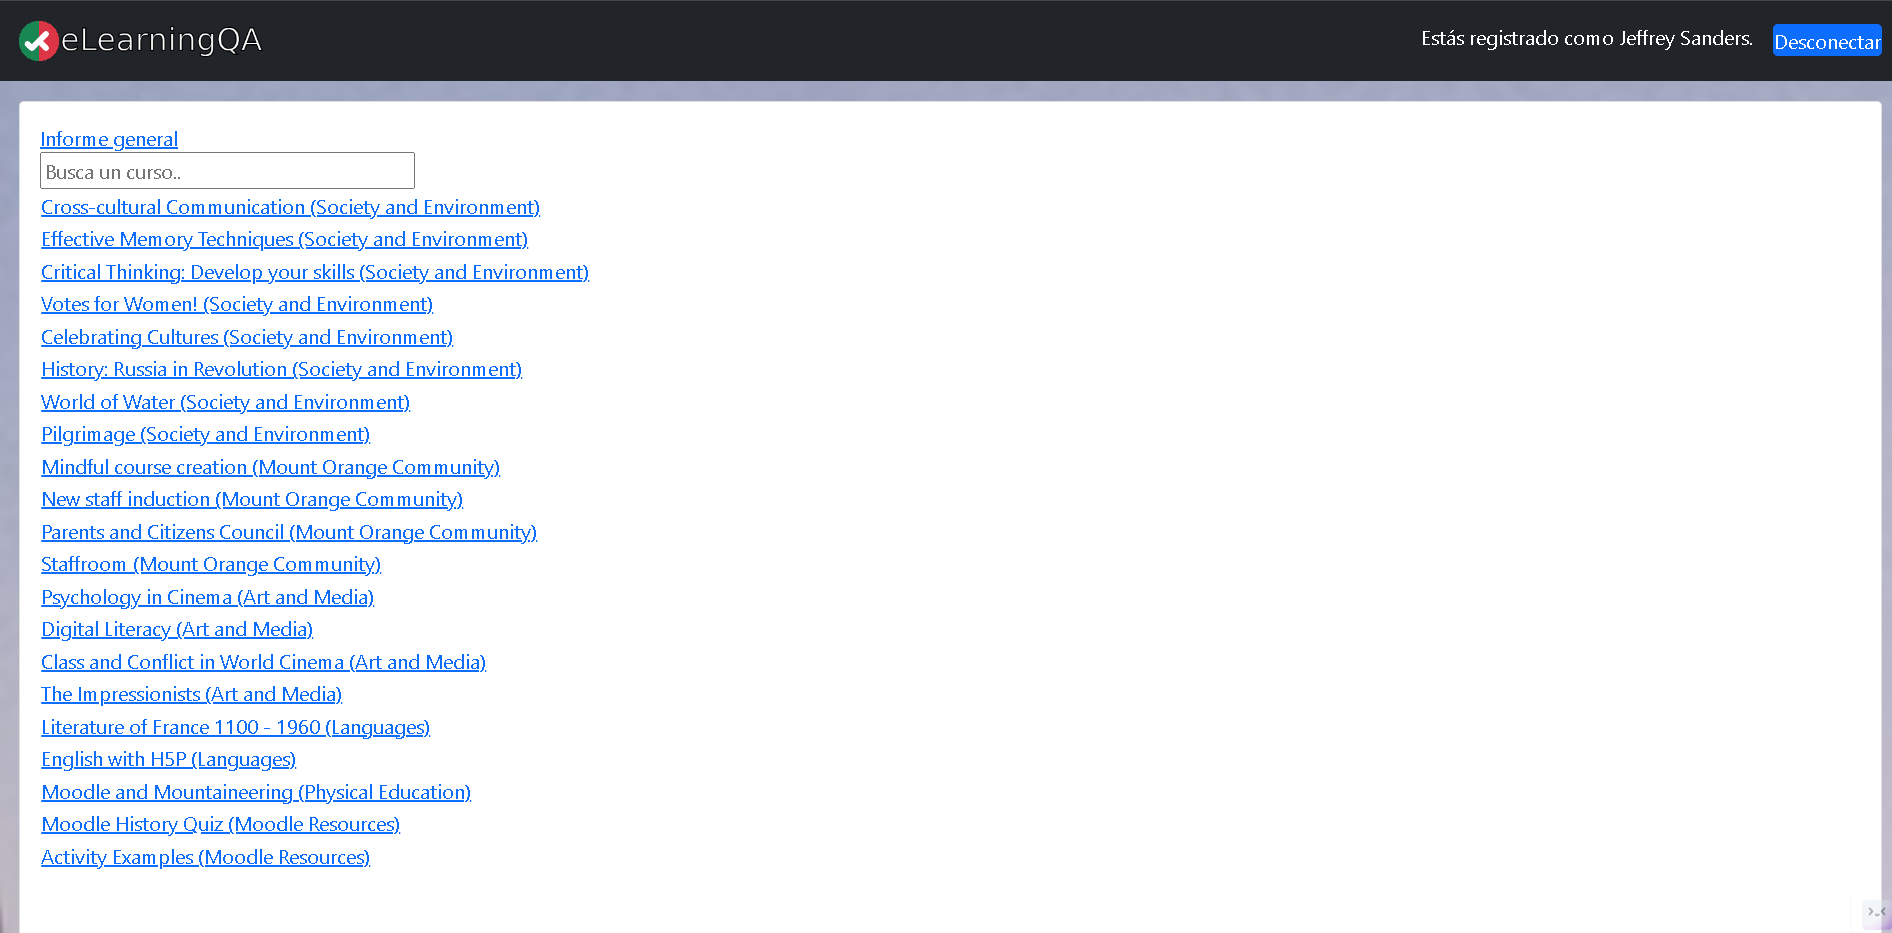
\includegraphics[width=1\linewidth]{img/lista-cursos.png}
            \caption{Lista de cursos}
            \label{fig:lista-cursos}
        \end{figure}
        \item \textbf{Informe de curso:} Una vez que se ha pulsado uno de los enlaces de la lista, se redirige a una pantalla con el informe generado \ref{fig:pantalla-informe}. Aquí se puede encontrar un marco con las reglas y las puntuaciones, un marco con las sugerencias para mejorar en aquellas reglas que hayan devuelto una puntuación negativa.  También, se pueden ver cuatro botones en la cabecera de la página, el primero para exportar un resumen del informe a Excel, el segundo con el informe de fases, el tercero para la redirección a la evolución del rendimiento y el último con un enlace que redirige al curso en Moodle.
            \begin{figure}[H]
                \centering
                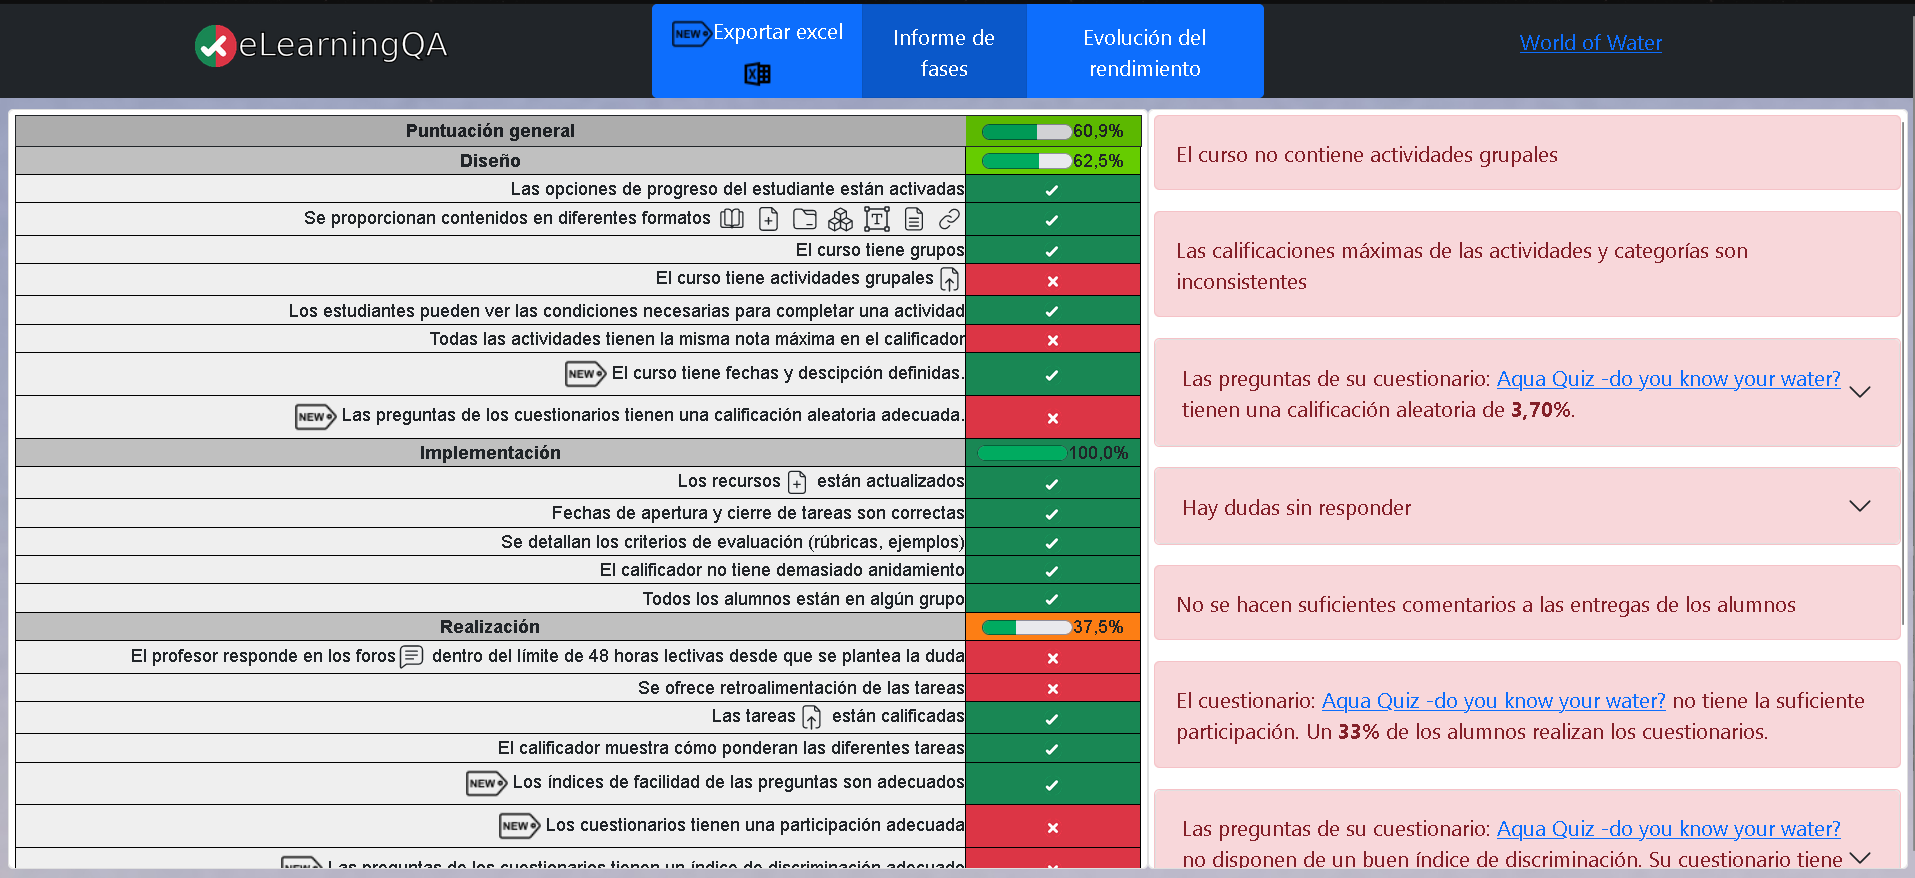
\includegraphics[width=1\linewidth]{img/pantalla_informe.png}
                \caption{Pantalla de informe de un curso}
                \label{fig:pantalla-informe}
            \end{figure} 
        \item \textbf{Evolución de rendimiento:} En la pantalla de evolución de rendimiento \ref{fig:evolucion-rendimiento} se podrá ver un gráfico con la evolución temporal de la calidad del curso, con base en los informes generados y un marco con las puntuaciones en las dimensiones de rol y perspectiva. 
        \begin{figure}[H]
            \centering
            \includegraphics[width=1\linewidth]{img/evolución-rendimiento.png}
            \caption{Pantalla de evolución de rendimiento}
            \label{fig:evolucion-rendimiento}
        \end{figure}
        \item \textbf{Documento Excel:} Cuando se pulsa el botón de exportación de Excel se descargará automáticamente un archivo Excel con un resumen del informe \ref{fig:informe-excel}.
            \begin{figure}[H]
                \centering
                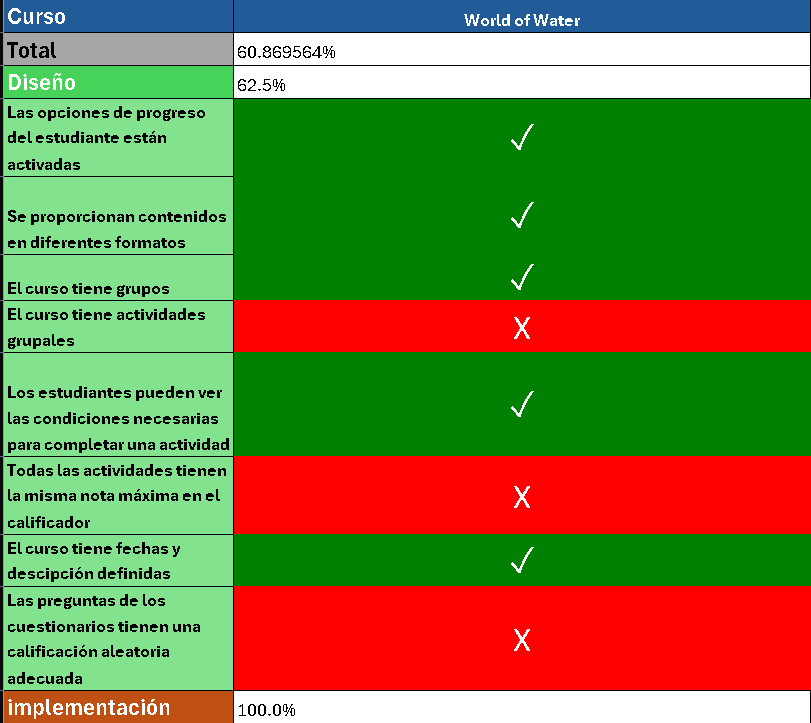
\includegraphics[width=1\linewidth]{img/informe_excel.png}
                \caption{Informe Excel}
                \label{fig:informe-excel}
            \end{figure}
        \item \textbf{Manual de usuario:} En esta pantalla se explican todas las funcionalidades de la aplicación informe \ref{fig:pantalla-manual}.
            \begin{figure}[H]
                \centering
                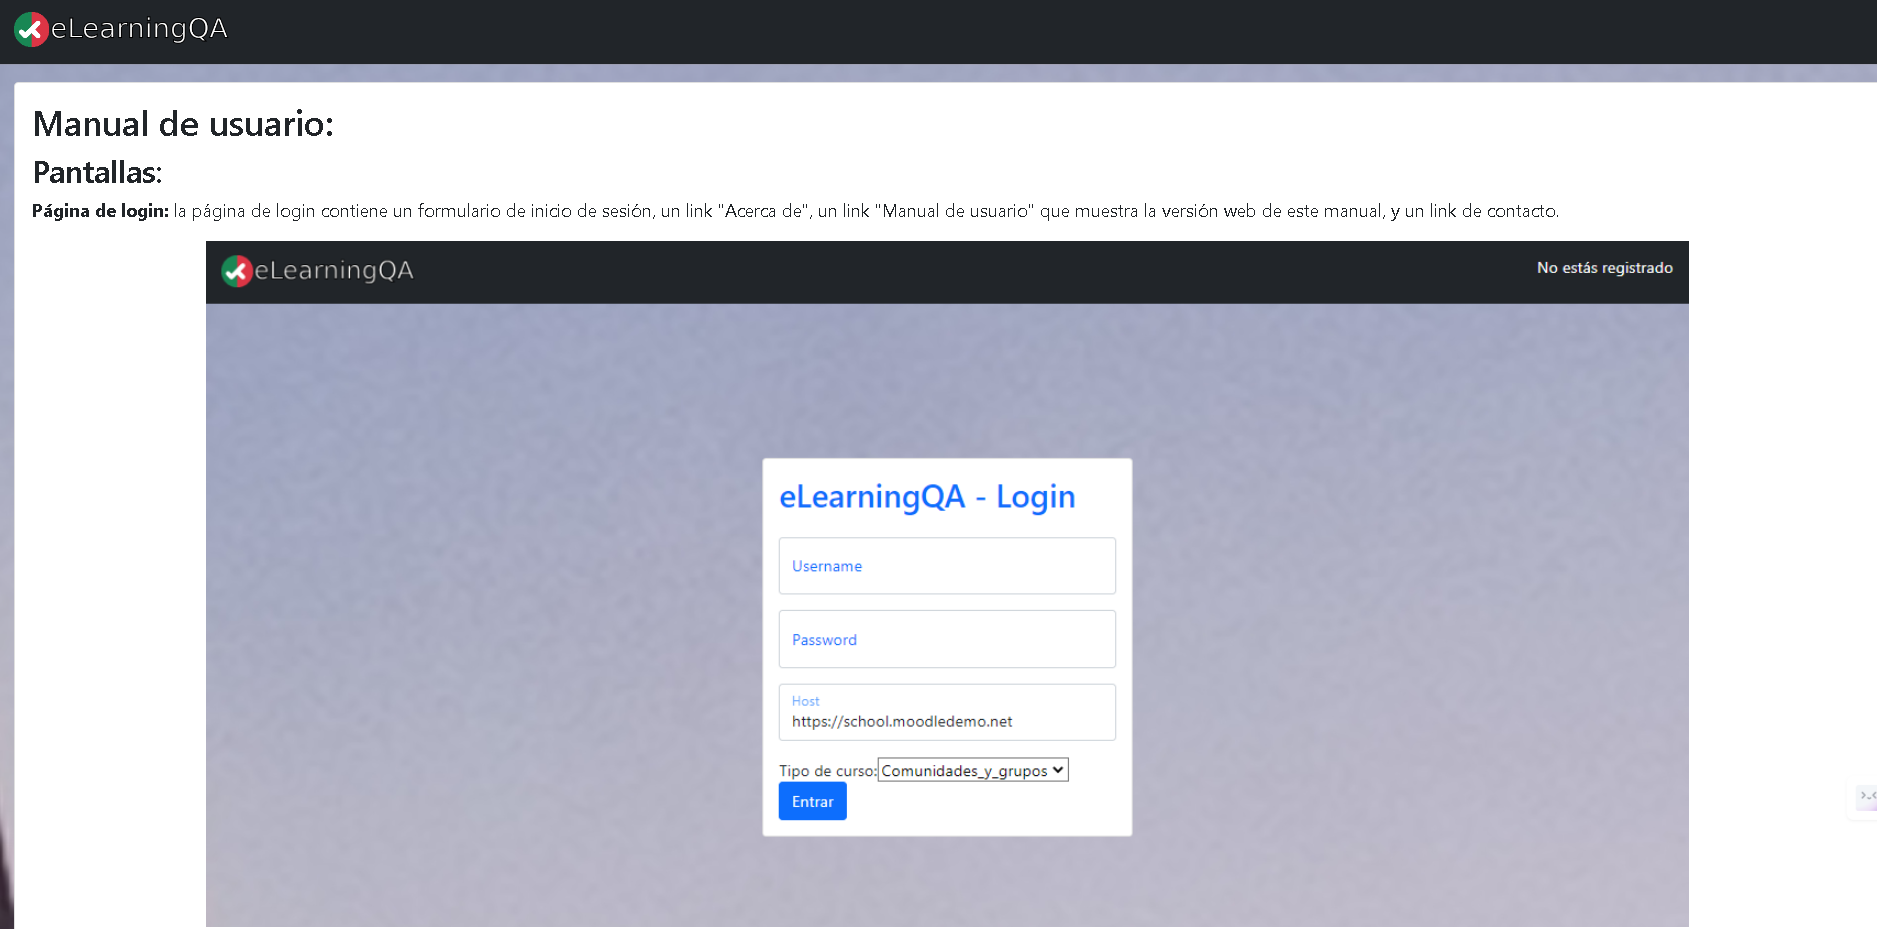
\includegraphics[width=1\linewidth]{img/pantalla_manual.png}
                \caption{Pantalla de manual de usuario}
                \label{fig:pantalla-manual}
            \end{figure}
        \item \textbf{Acerca de:} En esta pantalla se puede ver información relativa a licencias y responsables de la página \ref{fig:pantalla-about}.
            \begin{figure}[H]
                \centering
                
\includegraphics[width=1\linewidth]{img/pantalla_acerca.png}
                \caption{Pantalla de acerca de}
                \label{fig:pantalla-about}
            \end{figure}
        \item \textbf{Acerca de:} Al presionar el botón de ``contacto'', saldrá una ventana emergente del navegador para elegir opción para enviar el correo.
    \end{itemize}
        
\subsubsection{Acciones del usuario:}
    \begin{itemize}
    	\item
    	\textbf{Login:} para acceder a la aplicación son necesarias las
    	credenciales de acceso a una cuenta de la plataforma Moodle a la que
    	accede la aplicación (en el caso del prototipo es Mount Orange
    	School). Debe introducir su usuario y contraseña en los campos
    	``Username'' y ``Password''. Si quiere vaciar los campos, pulse el botón
    	``Borrar''. Para acceder a la página principal, pulse el botón ``Entrar''
    	tras haber introducido sus credenciales.
    	\item
    	\textbf{Desconectar:} desde la página principal, si desea finalizar su
    	sesión, pulse el botón ``Desconectar''. Esto invalidará sus credenciales
    	y le impedirá acceder a la aplicación hasta que se registre de nuevo
    	con unas credenciales válidas.
    	\item
    	\textbf{Generar informe específico:} la página principal muestra una
    	tabla con todos los cursos en los que se encuentra matriculado el
    	usuario registrado en formato de enlace. Al clicar un enlace, se
    	generará un informe en una pestaña aparte del navegador, que mostrará
    	los resultados del análisis que ha realizado la aplicación sobre el
    	curso correspondiente.
    	\item
    	\textbf{Generar informe global:} en la página principal hay un enlace
    	llamado ``Generar informe global''. Al hacer clic sobre este, se
    	generará un informe en una pestaña aparte del navegador que mostrará
    	un resumen de los análisis de todos los cursos en los que se encuentra
    	matriculado el profesor.
        \item
        \textbf{Exportar informes de Excel:} en la página del reporte de un curso, 
        hay un botón ``Exportar Excel'' en la cabecera de la página que permite exportar un resumen del
        informe generado a un archivo .xlsx.
        
    \end{itemize}
    
    \subsubsection{Explicación de las comprobaciones de los informes:}
    
    Las siguientes comprobaciones están relacionadas con los roles, fases, y
    perspectivas mencionadas anteriormente. Los distintos procesos del
    diseño instruccional se encuentran divididos en fases, ~con ciertas
    perspectivas en mente, y son responsabilidad directa o indirecta de
    ciertos roles. Al estar las comprobaciones ligadas a esos procesos se
    muestran agrupadas por fases, y después de la explicación se indican los
    roles responsables e involucrados, además de las perspectivas
    correspondientes.
    
    \textbf{Diseño:}
    
    \begin{itemize}
    	\item
    	\textbf{Las opciones de progreso del estudiante están activadas}: se
    	comprueba que estén habilitadas las opciones de progreso de los
    	estudiantes en el curso.~{Responsable:} Diseñador
    	{Involucrados:} Facilitador {Perspectivas:} Pedagógica
    	\item
    	\textbf{Se proporcionan contenidos en diferentes formatos:} se
    	comprueba que haya variedad de formatos en los recursos del curso.
    	{Responsable:} Diseñador {Involucrados:} Facilitador y
    	Proveedor {Perspectivas:} Pedagógica y Tecnológica
    	\item
    	\textbf{El curso tiene grupos:} se comprueba que existan grupos
    	definidos en el curso. {Responsable:} Diseñador
    	{Involucrados:} Facilitador y Proveedor {Perspectivas:}
    	Pedagógica
    	\item
    	\textbf{El curso tiene actividades grupales:} se comprueba que existan
    	actividades con entrega grupal habilitada en el curso.
    	{Responsable:} Diseñador {Involucrados:} Facilitador y
    	Proveedor {Perspectivas:} Pedagógica
    	\item
    	\textbf{Los estudiantes pueden ver las condiciones necesarias para
    		completar una actividad:} se comprueba que esté habilitada la opción
    	de mostrar las condiciones para completar una actividad en el curso.
    	{Responsable:} Diseñador {Involucrados:} Facilitador y
    	Proveedor {Perspectivas:} Pedagógica
    	\item
    	\textbf{Todas las actividades tienen la misma nota máxima en el
    		calificador:} se comprueba que exista una consistencia en las notas
    	máximas de los ítems de calificación (tareas, entregas, cuestionarios)
    	del curso. {Responsable:} Diseñador {Involucrados:}
    	Facilitador y Proveedor {Perspectivas:} Pedagógica
        \item 
        \textbf{El curso tiene fechas y descripción definidas:} se comprueba que estén definidas las fechas de inicio y fin del curso, así como una descripción. {Responsable:} Diseñador {Involucrados:} Facilitador y Proveedor {Perspectivas:} Pedagógica y Estratégica
        \item 
        \textbf{Las preguntas de los cuestionarios tienen una calificación aleatoria adecuada:} se comprueba que el índice de calificación aleatoria de los cuestionarios este por debajo de un valor definido. {Responsable:} Diseñador {Involucrados:} Facilitador {Perspectivas:} Pedagógica
    \end{itemize}
    
    \textbf{Implementación:}
    
    \begin{itemize}
    	\item
    	\textbf{Los recursos están actualizados:} se comprueba que los
    	recursos del curso tengan una fecha de creación reciente.
    	{Responsable:} Diseñador {Involucrados:} Facilitador y
    	Proveedor {Perspectivas:} Pedagógica y Tecnológica
    	\item
    	\textbf{Fechas de apertura y cierre de tareas son correctas:} se
    	comprueba que las fechas de apertura y cierre de tareas y
    	cuestionarios no se solapen de forma errónea con las fechas de inicio
    	y fin del curso. {Responsable:} Facilitador
    	{Involucrados:} Diseñador y Proveedor {Perspectivas:}
    	Pedagógica y Tecnológica
    	\item
    	\textbf{Se detallan los criterios de evaluación:} se comprueba que
    	exista en al menos una actividad una rúbrica o una guía de calificación
    	en el curso.~{Responsable:} Diseñador {Involucrados:}
    	Facilitador y Proveedor {Perspectivas:} Pedagógica y Tecnológica
    	\item
    	\textbf{El calificador no tiene demasiado anidamiento:} se comprueba
    	que la estructura de las categorías del calificador no sea demasiado
    	enrevesada. {Responsable:} Diseñador {Involucrados:}
    	Facilitador y Proveedor {Perspectivas:} Pedagógica y Estratégica
    	\item
    	\textbf{Todos los alumnos están en algún grupo:} se comprueba que cada
    	alumno pertenezca a un grupo. {Responsable:} Proveedor
    	{Involucrados:} Diseñador {Perspectivas:} Tecnológica y
    	Estratégica
    \end{itemize}
    
    \textbf{Realización:}
    
    \begin{itemize}
    	\item
    	\textbf{El profesor responde en los foros dentro del límite de 48
    		horas lectivas desde que se plantea la duda:} se comprueba que no
    	haya preguntas por parte de alumnos que estén sin responder en un
    	tiempo razonable. {Responsable:} Facilitador
    	{Involucrados:} Diseñador y Proveedor {Perspectivas:}
    	Pedagógica y Tecnológica
    	\item
    	\textbf{Se ofrece retroalimentación de las tareas:} se comprueba que
    	el profesor deje comentarios en la mayoría de calificaciones que haga.
    	{Responsable:} Facilitador {Involucrados:} Diseñador y
    	Proveedor {Perspectivas:} Pedagógica y Tecnológica
    	\item
    	\textbf{Las tareas están calificadas:} se comprueba que no haya
    	entregas de alumnos que hayan pasado una semana sin calificación.
    	{Responsable:} Facilitador {Involucrados:} Diseñador y
    	Proveedor {Perspectivas:} Pedagógica y Tecnológica
    	\item
    	\textbf{El calificador muestra cómo ponderan las diferentes tareas:}
    	se comprueba que el calificador muestre los pesos de los ítems de
    	calificación. {Responsable:} Facilitador {Involucrados:}
    	Diseñador y Proveedor {Perspectivas:} Pedagógica y Tecnológica
        \item
        \textbf{Los índices de facilidad de las preguntas son adecuados:} se comprueba que los índices de facilidad de las preguntas de los cuestionarios estén dentro de los intervalos definidos.  {Responsable:} Facilitador {Involucrados:} Diseñador y Proveedor {Perspectivas:} Pedagógica, Estratégica y Tecnológica
        \item
        \textbf{Los cuestionarios tienen una participación adecuada:} se comprueba que la participación de los cuestionarios sea superior a un valor definido. {Responsable:} Facilitador {Involucrados:} Diseñador y Proveedor {Perspectivas:} Pedagógica, Estratégica y Tecnológica
        \item
        \textbf{Las preguntas de los cuestionarios tienen un índice de discriminación adecuado:} se comprueba que los índices de discriminación de las preguntas estén por encima de un valor definido. {Responsable:} Facilitador {Involucrados:} Diseñador y Proveedor {Perspectivas:} Pedagógica, Estratégica y Tecnológica  
        \item
        \textbf{Los cuestionarios tienen un coeficiente de consistencia interna adecuado:} se comprueba que los coeficientes de consistencia interna estén por encima de un valor definido. {Responsable:} Facilitador {Involucrados:} Diseñador y Proveedor {Perspectivas:} Pedagógica, Estratégica y Tecnológica  
    \end{itemize}
    
    \textbf{Evaluación:}
    
    \begin{itemize}
    	\item
    	\textbf{La mayoría de alumnos responden a los feedbacks:} se comprueba
    	que no haya muchos alumnos que no respondan a los feedbacks.
    	{Responsable:} Proveedor {Involucrados:} Diseñador y
    	Facilitador {Perspectivas:} Pedagógica, Tecnológica, y
    	Estratégica
    	\item
    	\textbf{Se utilizan encuestas de opinión:} se comprueba que el curso
    	contenga encuestas de opinión. {Responsable:} Proveedor
    	{Involucrados:} Diseñador y Facilitador {Perspectivas:}
    	Pedagógica, Tecnológica, y Estratégica
    \end{itemize}
    
    